\chapter{Modelo Conceptual}
\clearpage

\section {Modelo de Clases}
\par En este documento se presenta el diagrama de clases generado sobre el sistema de seguridad al volante que está siendo desarrollado para CARSAFETY. El diagrama, representado con notación UML (Unified Modeling Language), muestra la estructura del sistema, especificando sus diferentes clases, atributos y métodos.


%Figura
\begin{figure}[H]
\begin{center}
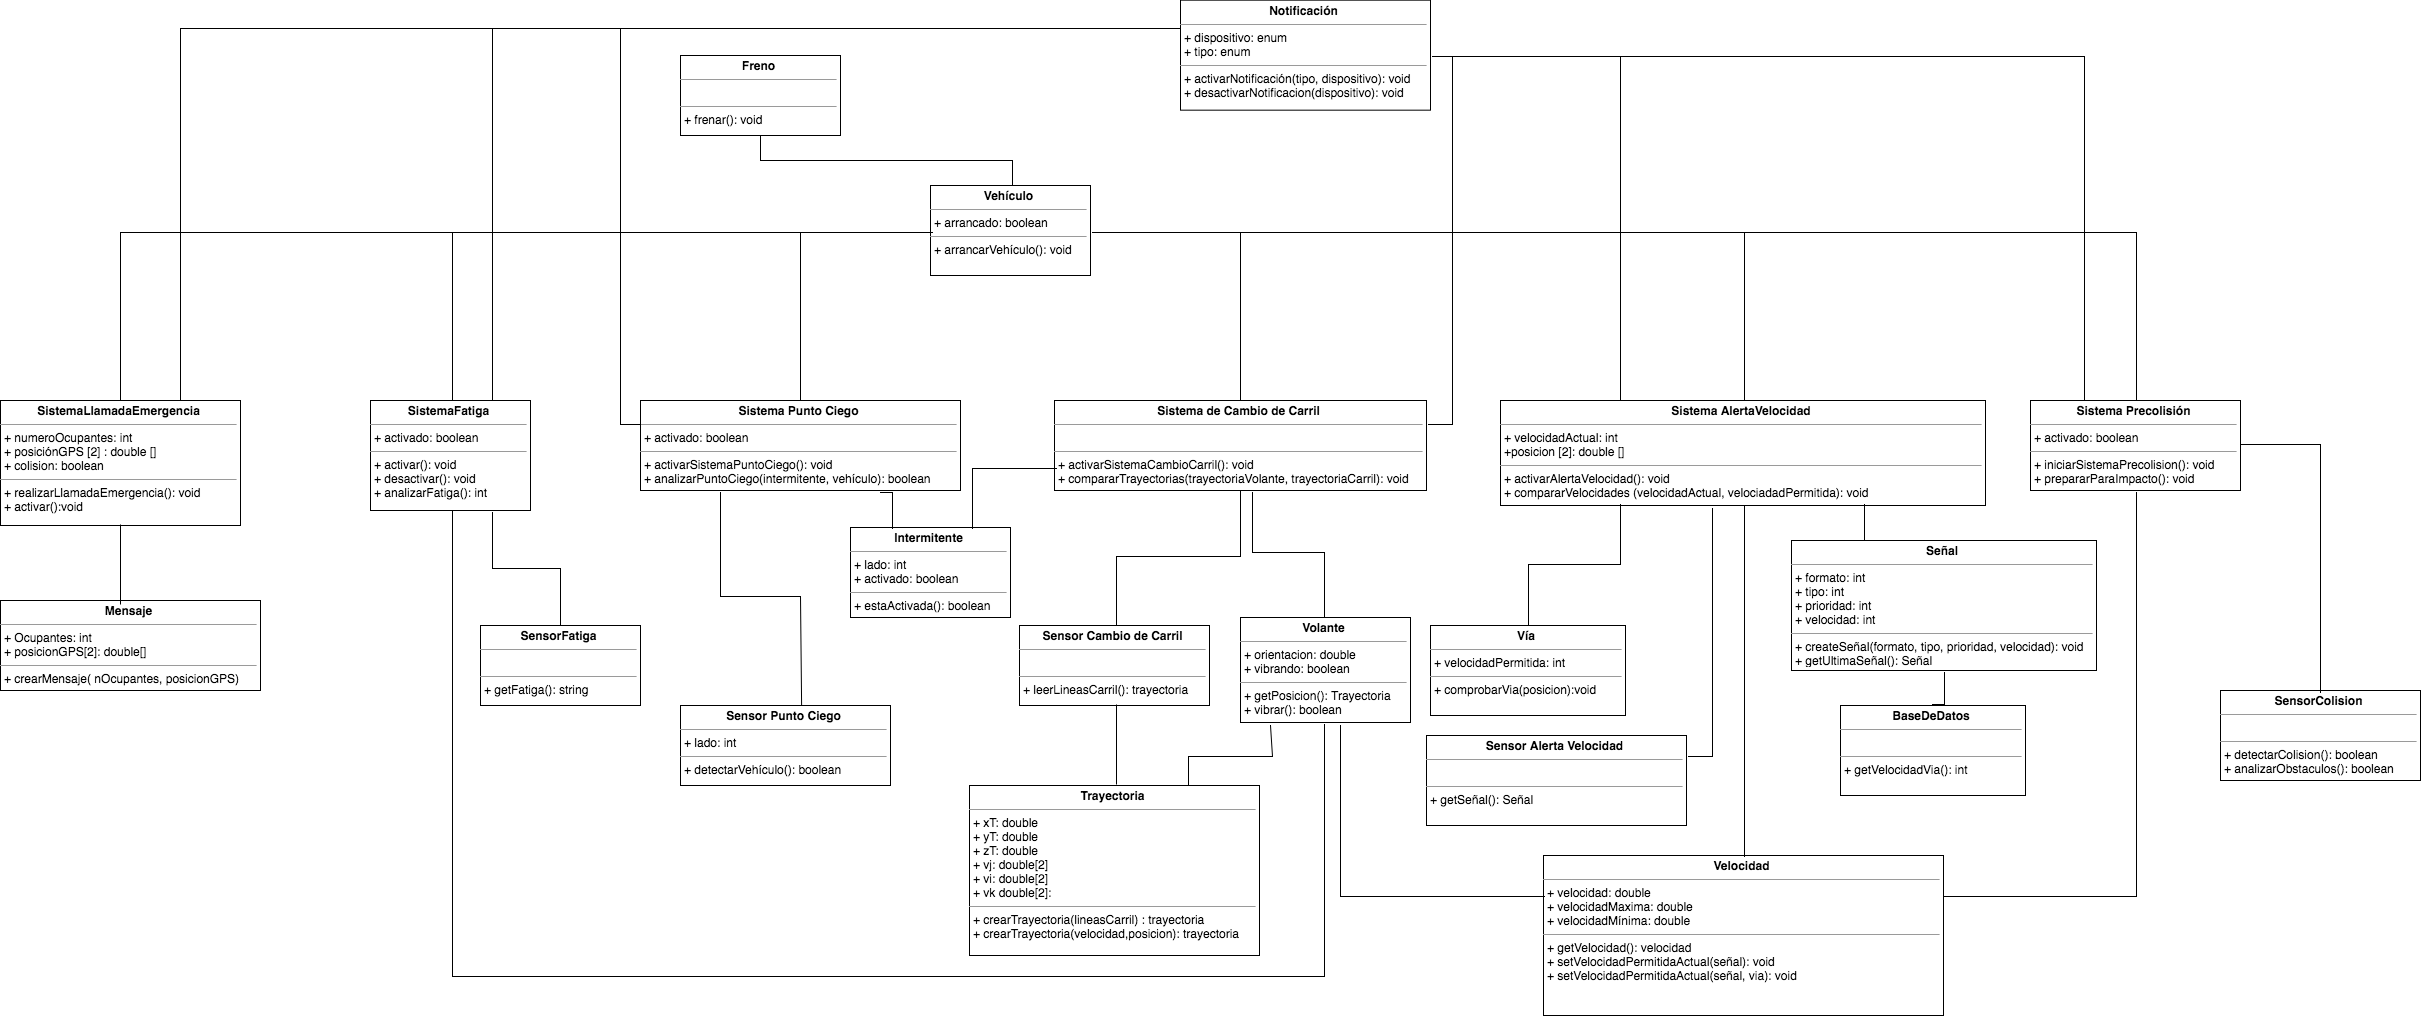
\includegraphics[width=1\textwidth]{./img/m_clases.png}
\end{center}
\caption{Modelo de Clases}
\label{tab:m_clases}
\end{figure}

\par Debido a la extensión del diagrama, hemos procedido a subsividirlo en función de los subsistemas involucrados. Todos los subsistemas se relacionan con las clases Vehículo \ref{tab:c_vehiculo} y Notificación \ref{tab:c_Notificacion}.

%Figura
\begin{figure}[H]
\begin{center}
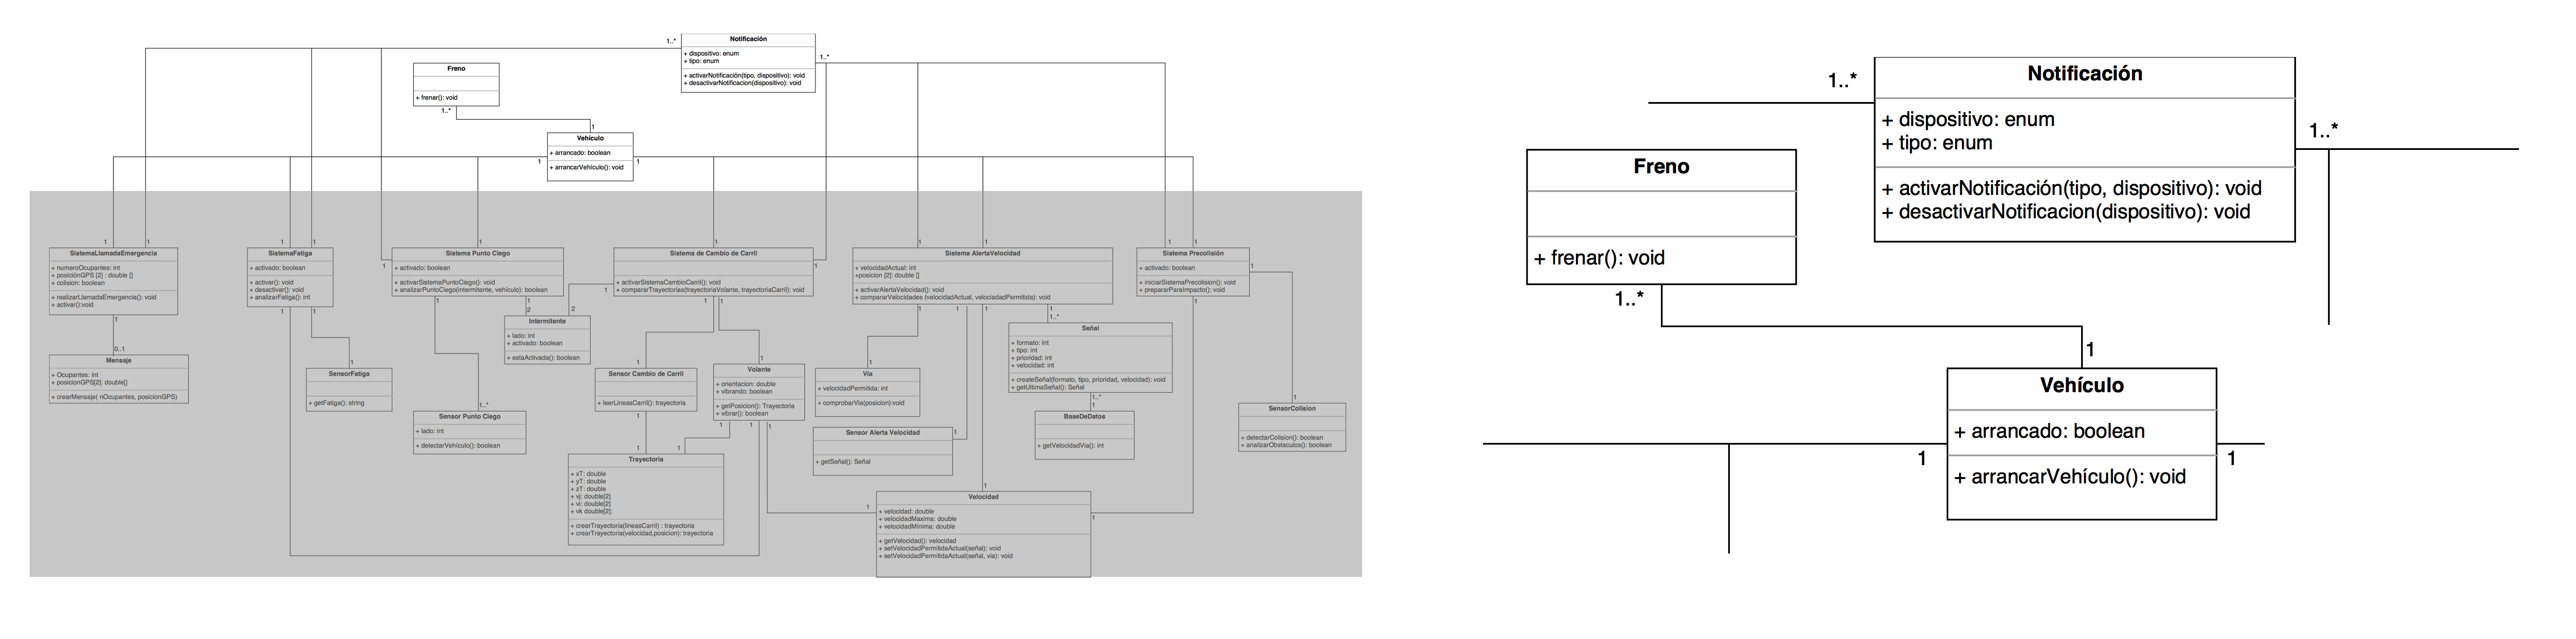
\includegraphics[width=1\textwidth]{./img/VehiculoNotificacion.png}
\end{center}
\caption{Clases Vehiculo, Notificación}
\label{tab:c_vehiculo_notificacionPNG}
\end{figure}

%Figura
\begin{figure}[H]
\begin{center}
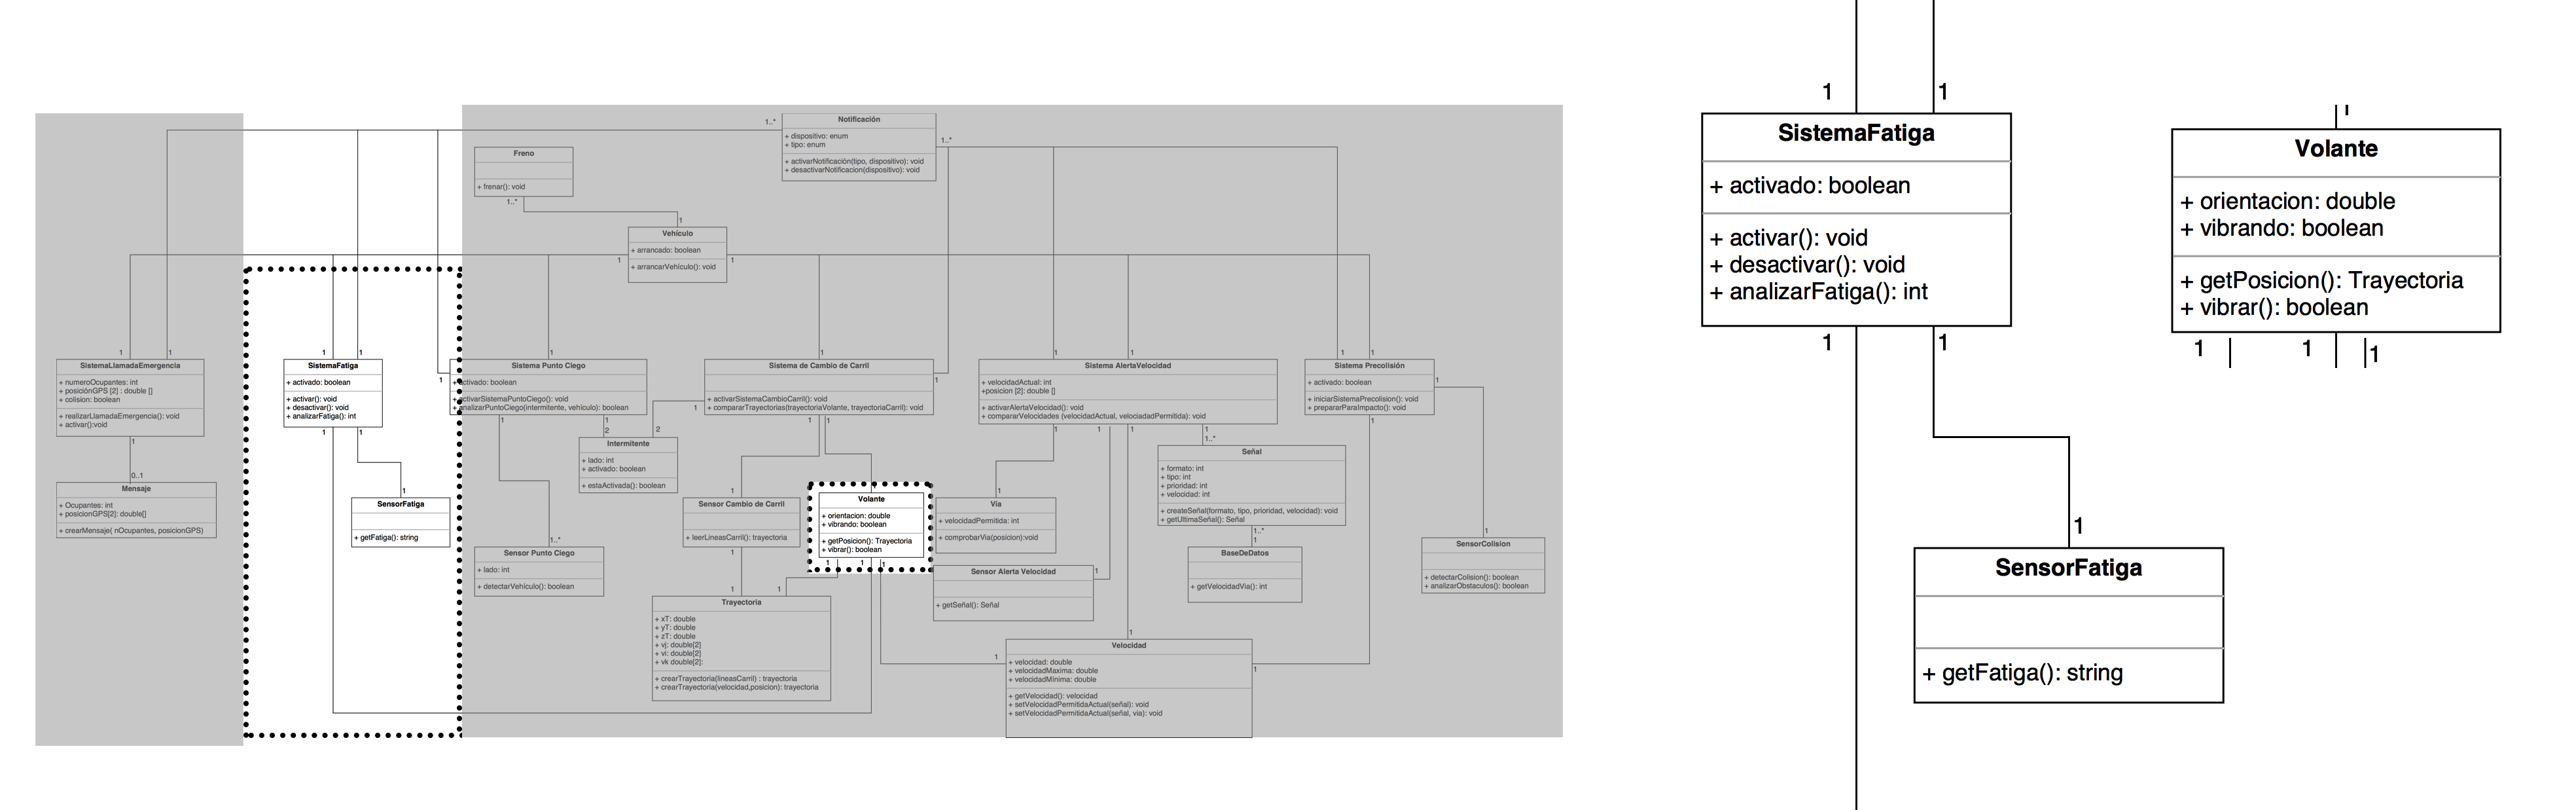
\includegraphics[width=1\textwidth]{./img/SistemaFatiga.png}
\end{center}
\caption{Clases pertenecientes al subsistema SistemaFatiga}
\label{tab:c_SistemaFatigaPNG}
\end{figure}

%Figura
\begin{figure}[H]
\begin{center}
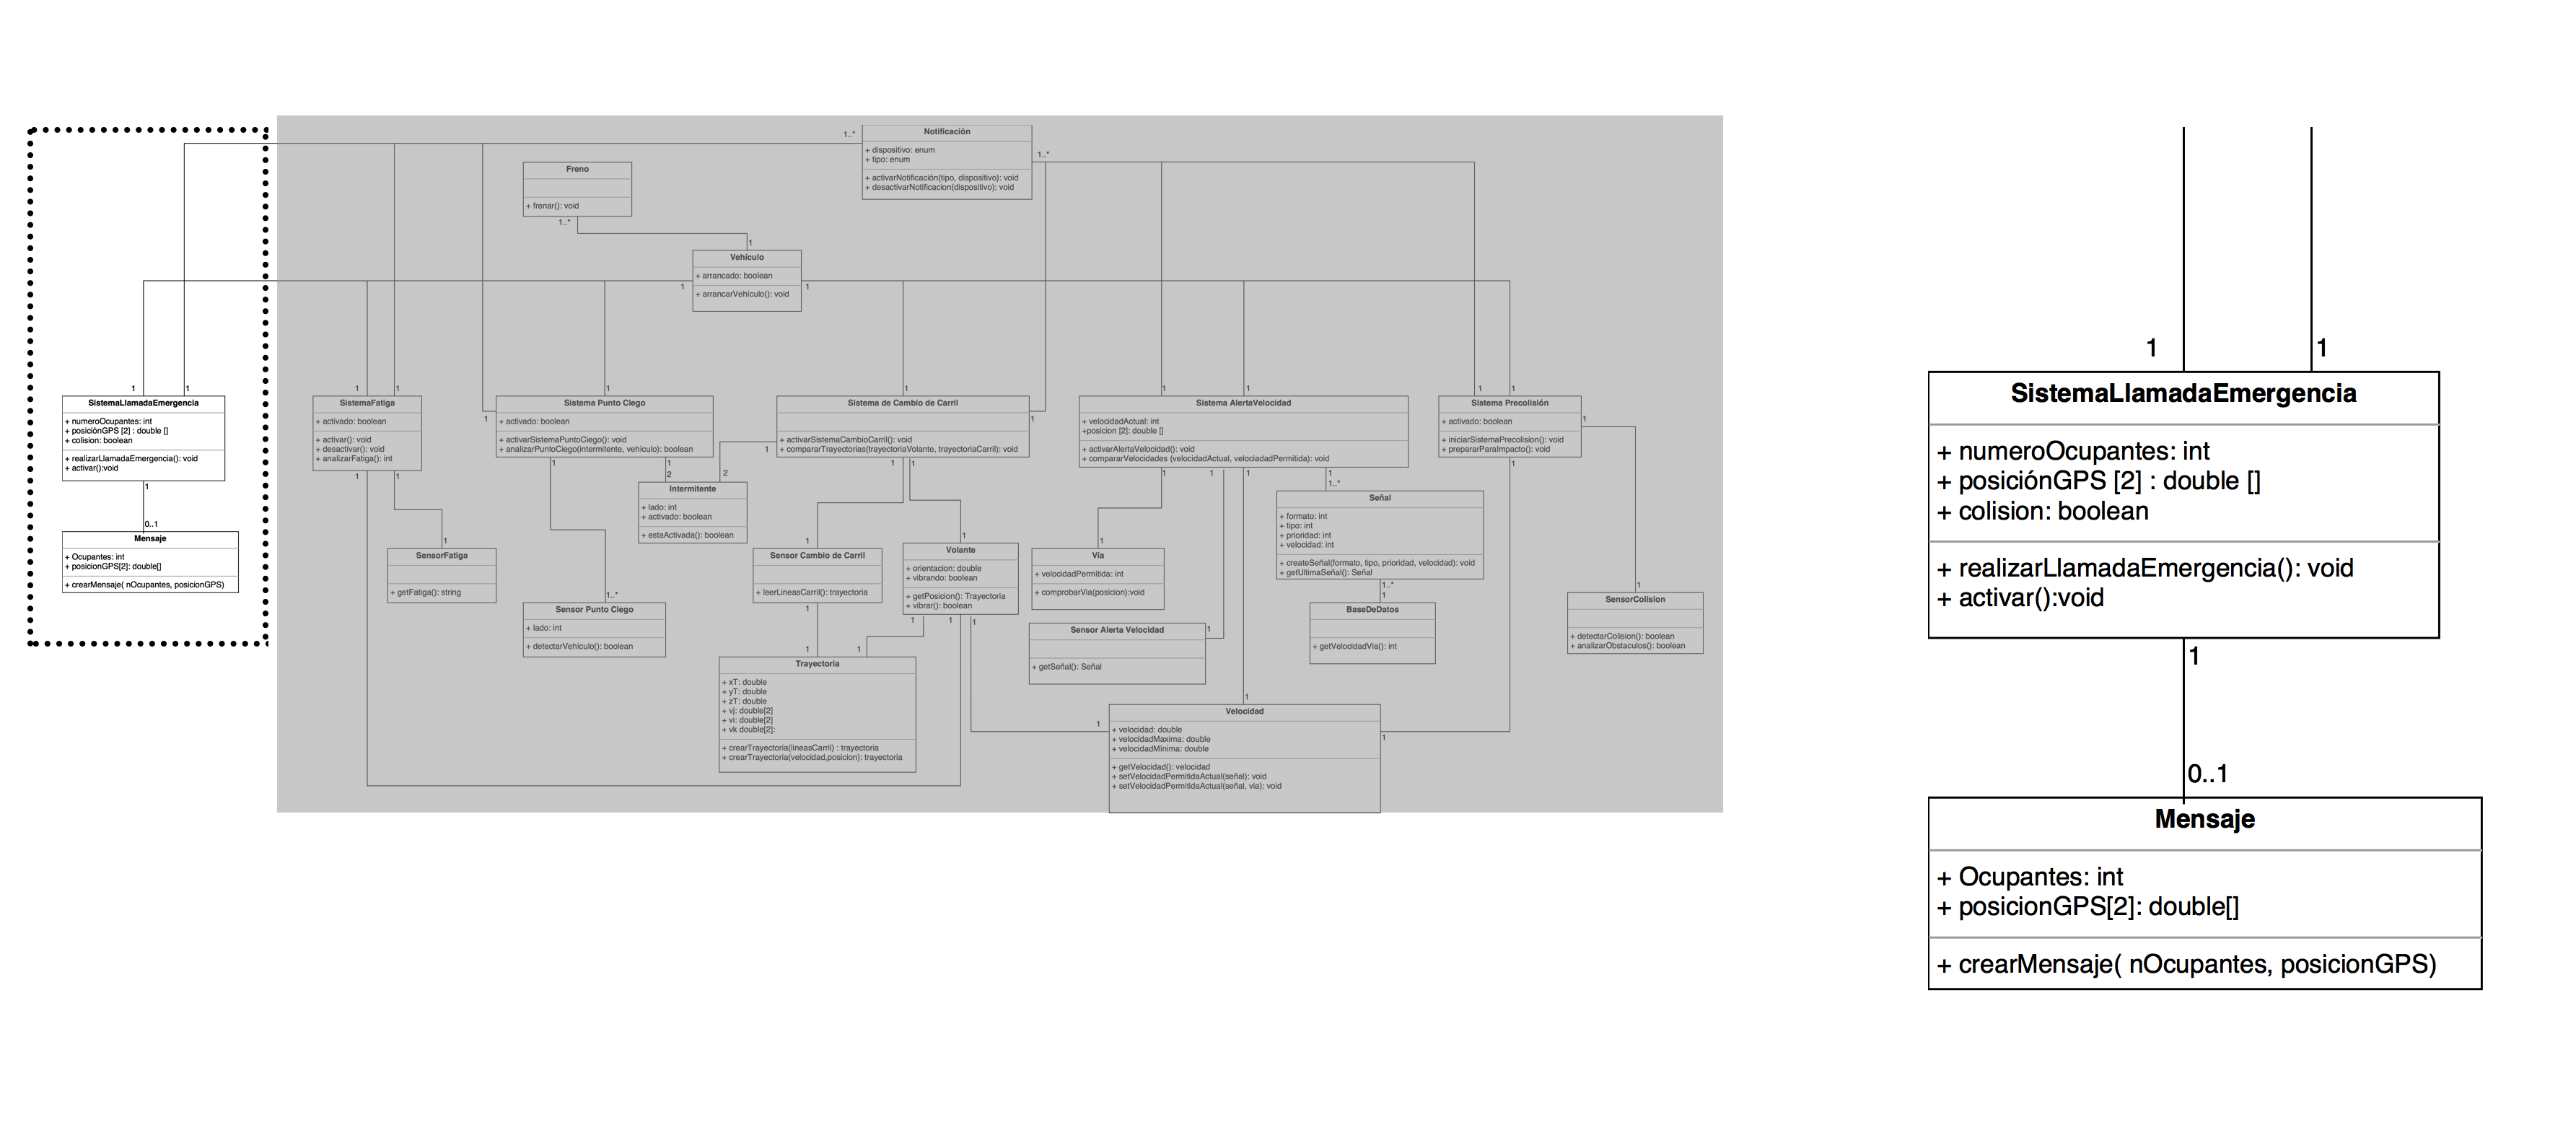
\includegraphics[width=1\textwidth]{./img/SistemaLlamadaEmergencia.png}
\end{center}
\caption{Clases pertenecientes al subsistema SistemaLlamadaEmergencia}
\label{tab:c_SistemaLlamadaEmergenciaPNG}
\end{figure}



%Figura
\begin{figure}[H]
\begin{center}
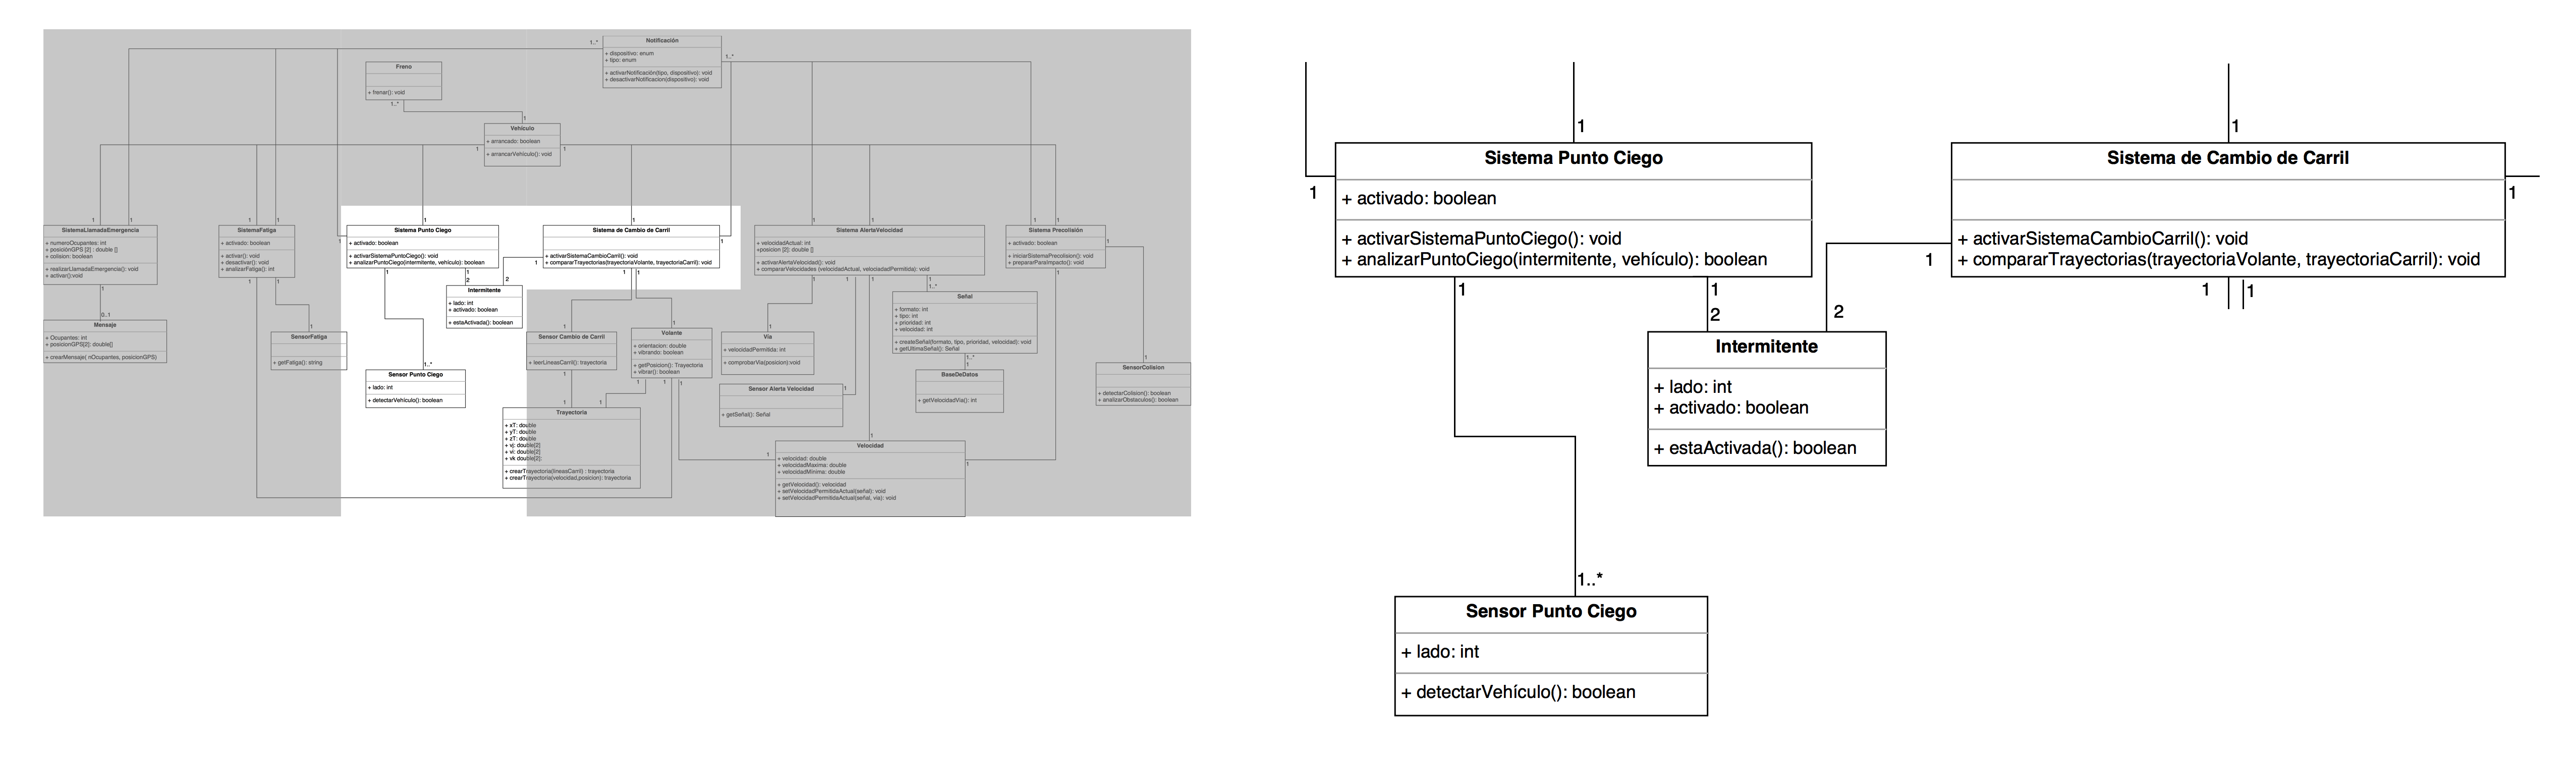
\includegraphics[width=1\textwidth]{./img/SistemaPuntoCiego.png}
\end{center}
\caption{Clases pertenecientes al subsistema SistemaPuntoCiego}
\label{tab:c_SistemaPuntoCiegoPNG}
\end{figure}


%Figura
\begin{figure}[h]
\begin{center}
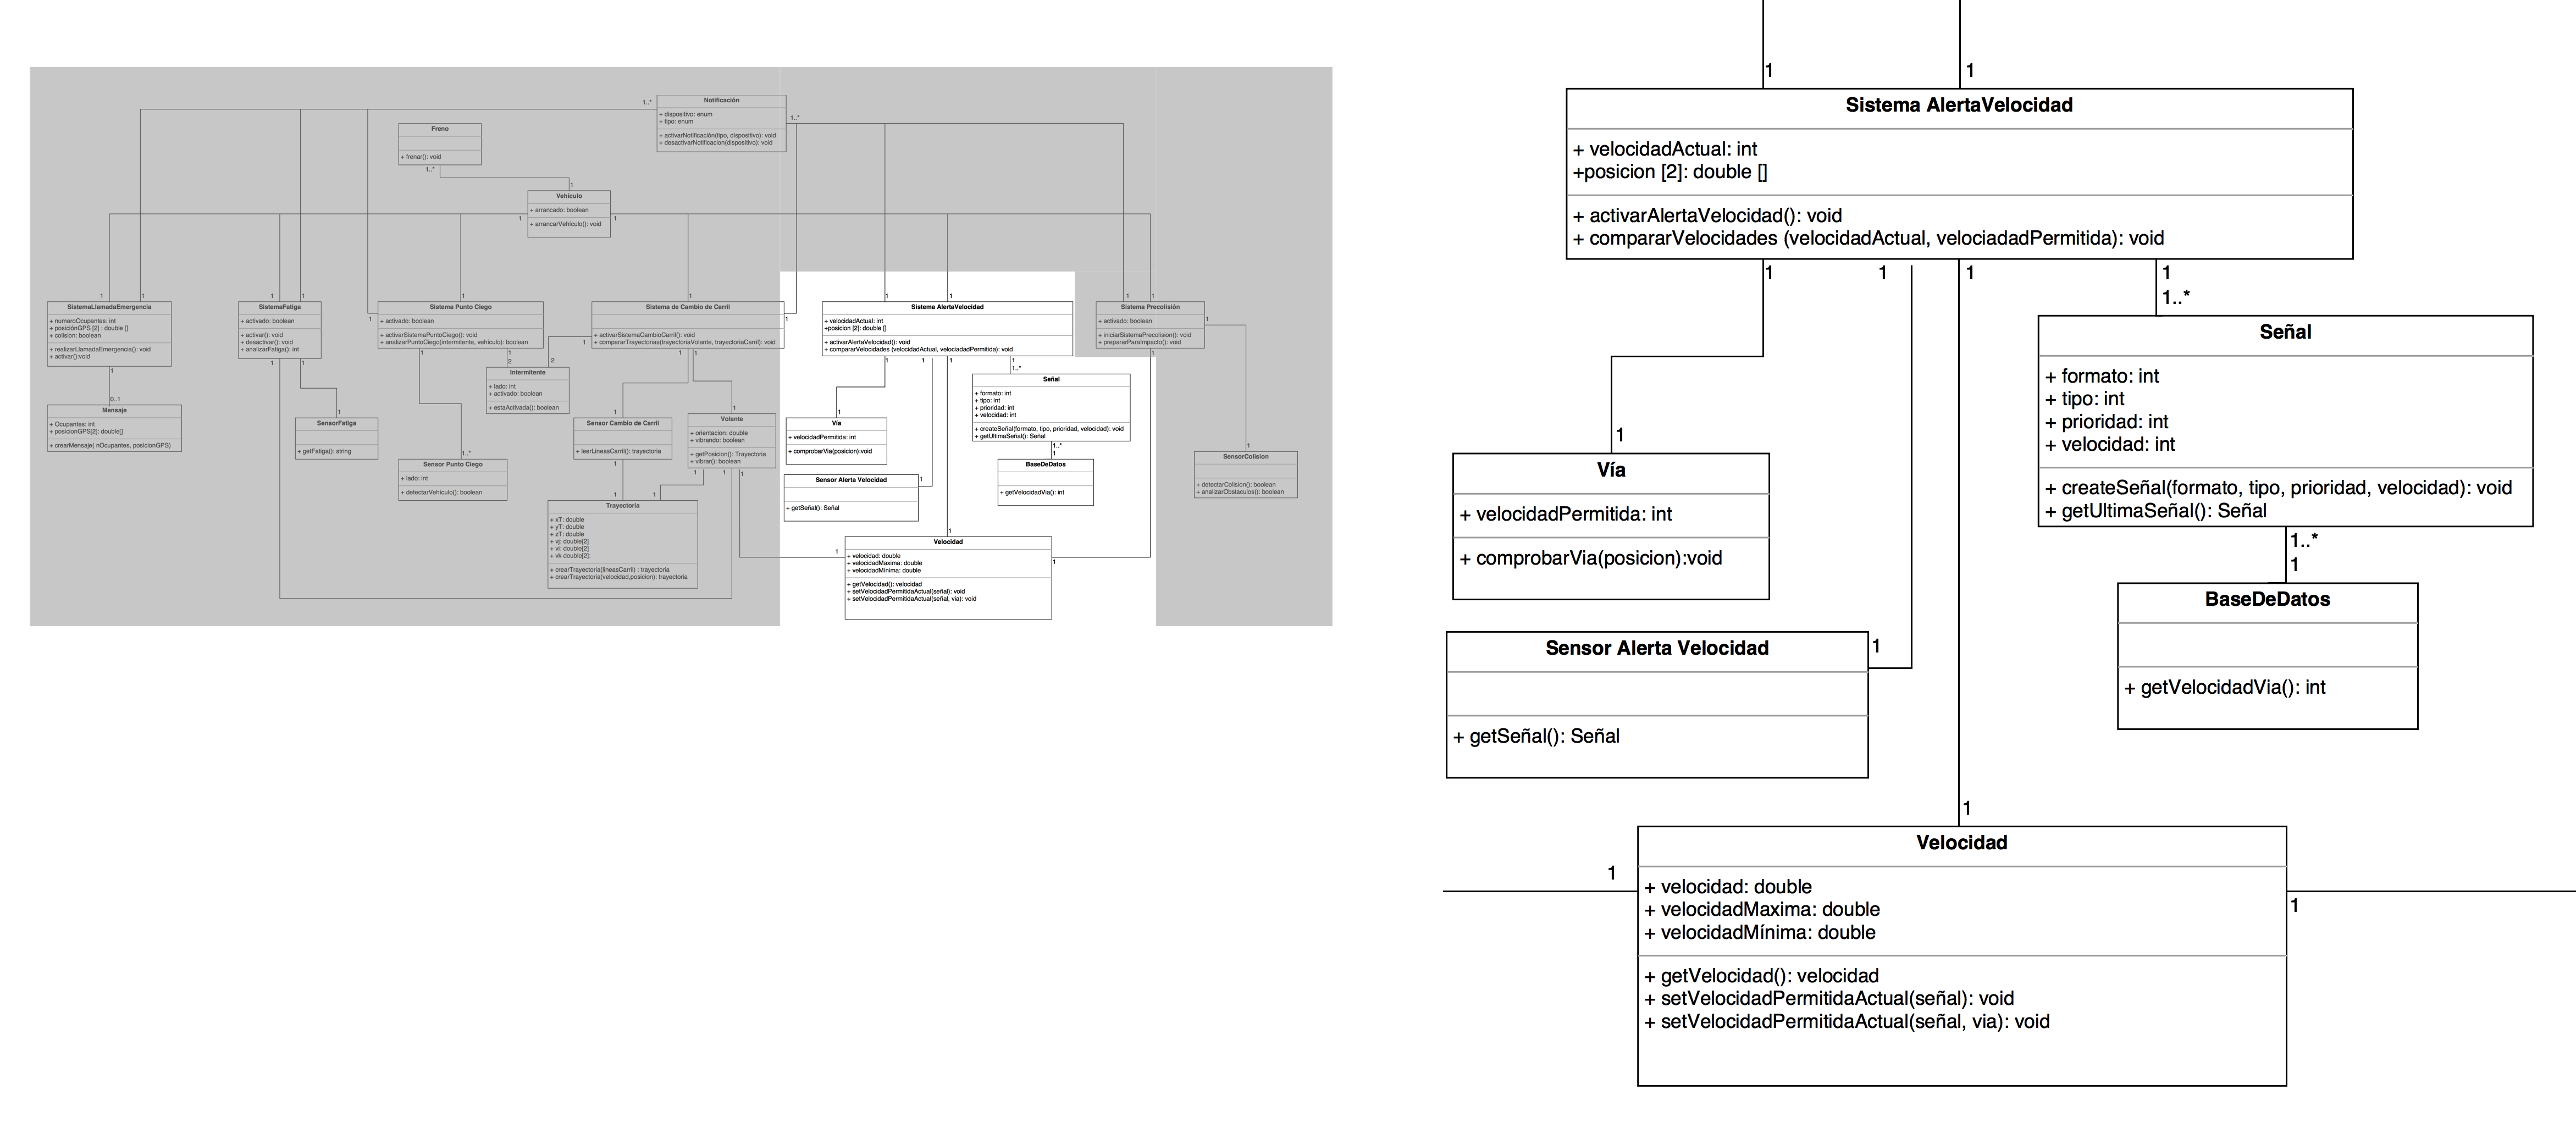
\includegraphics[width=1\textwidth]{./img/SistemaVelocidad.png}
\end{center}
\caption{Clases pertenecientes al subsistema SistemaVelocidad}
\label{tab:c_SistemaVelocidadPNG}
\end{figure}

%Figura
\begin{figure}[H]
\begin{center}
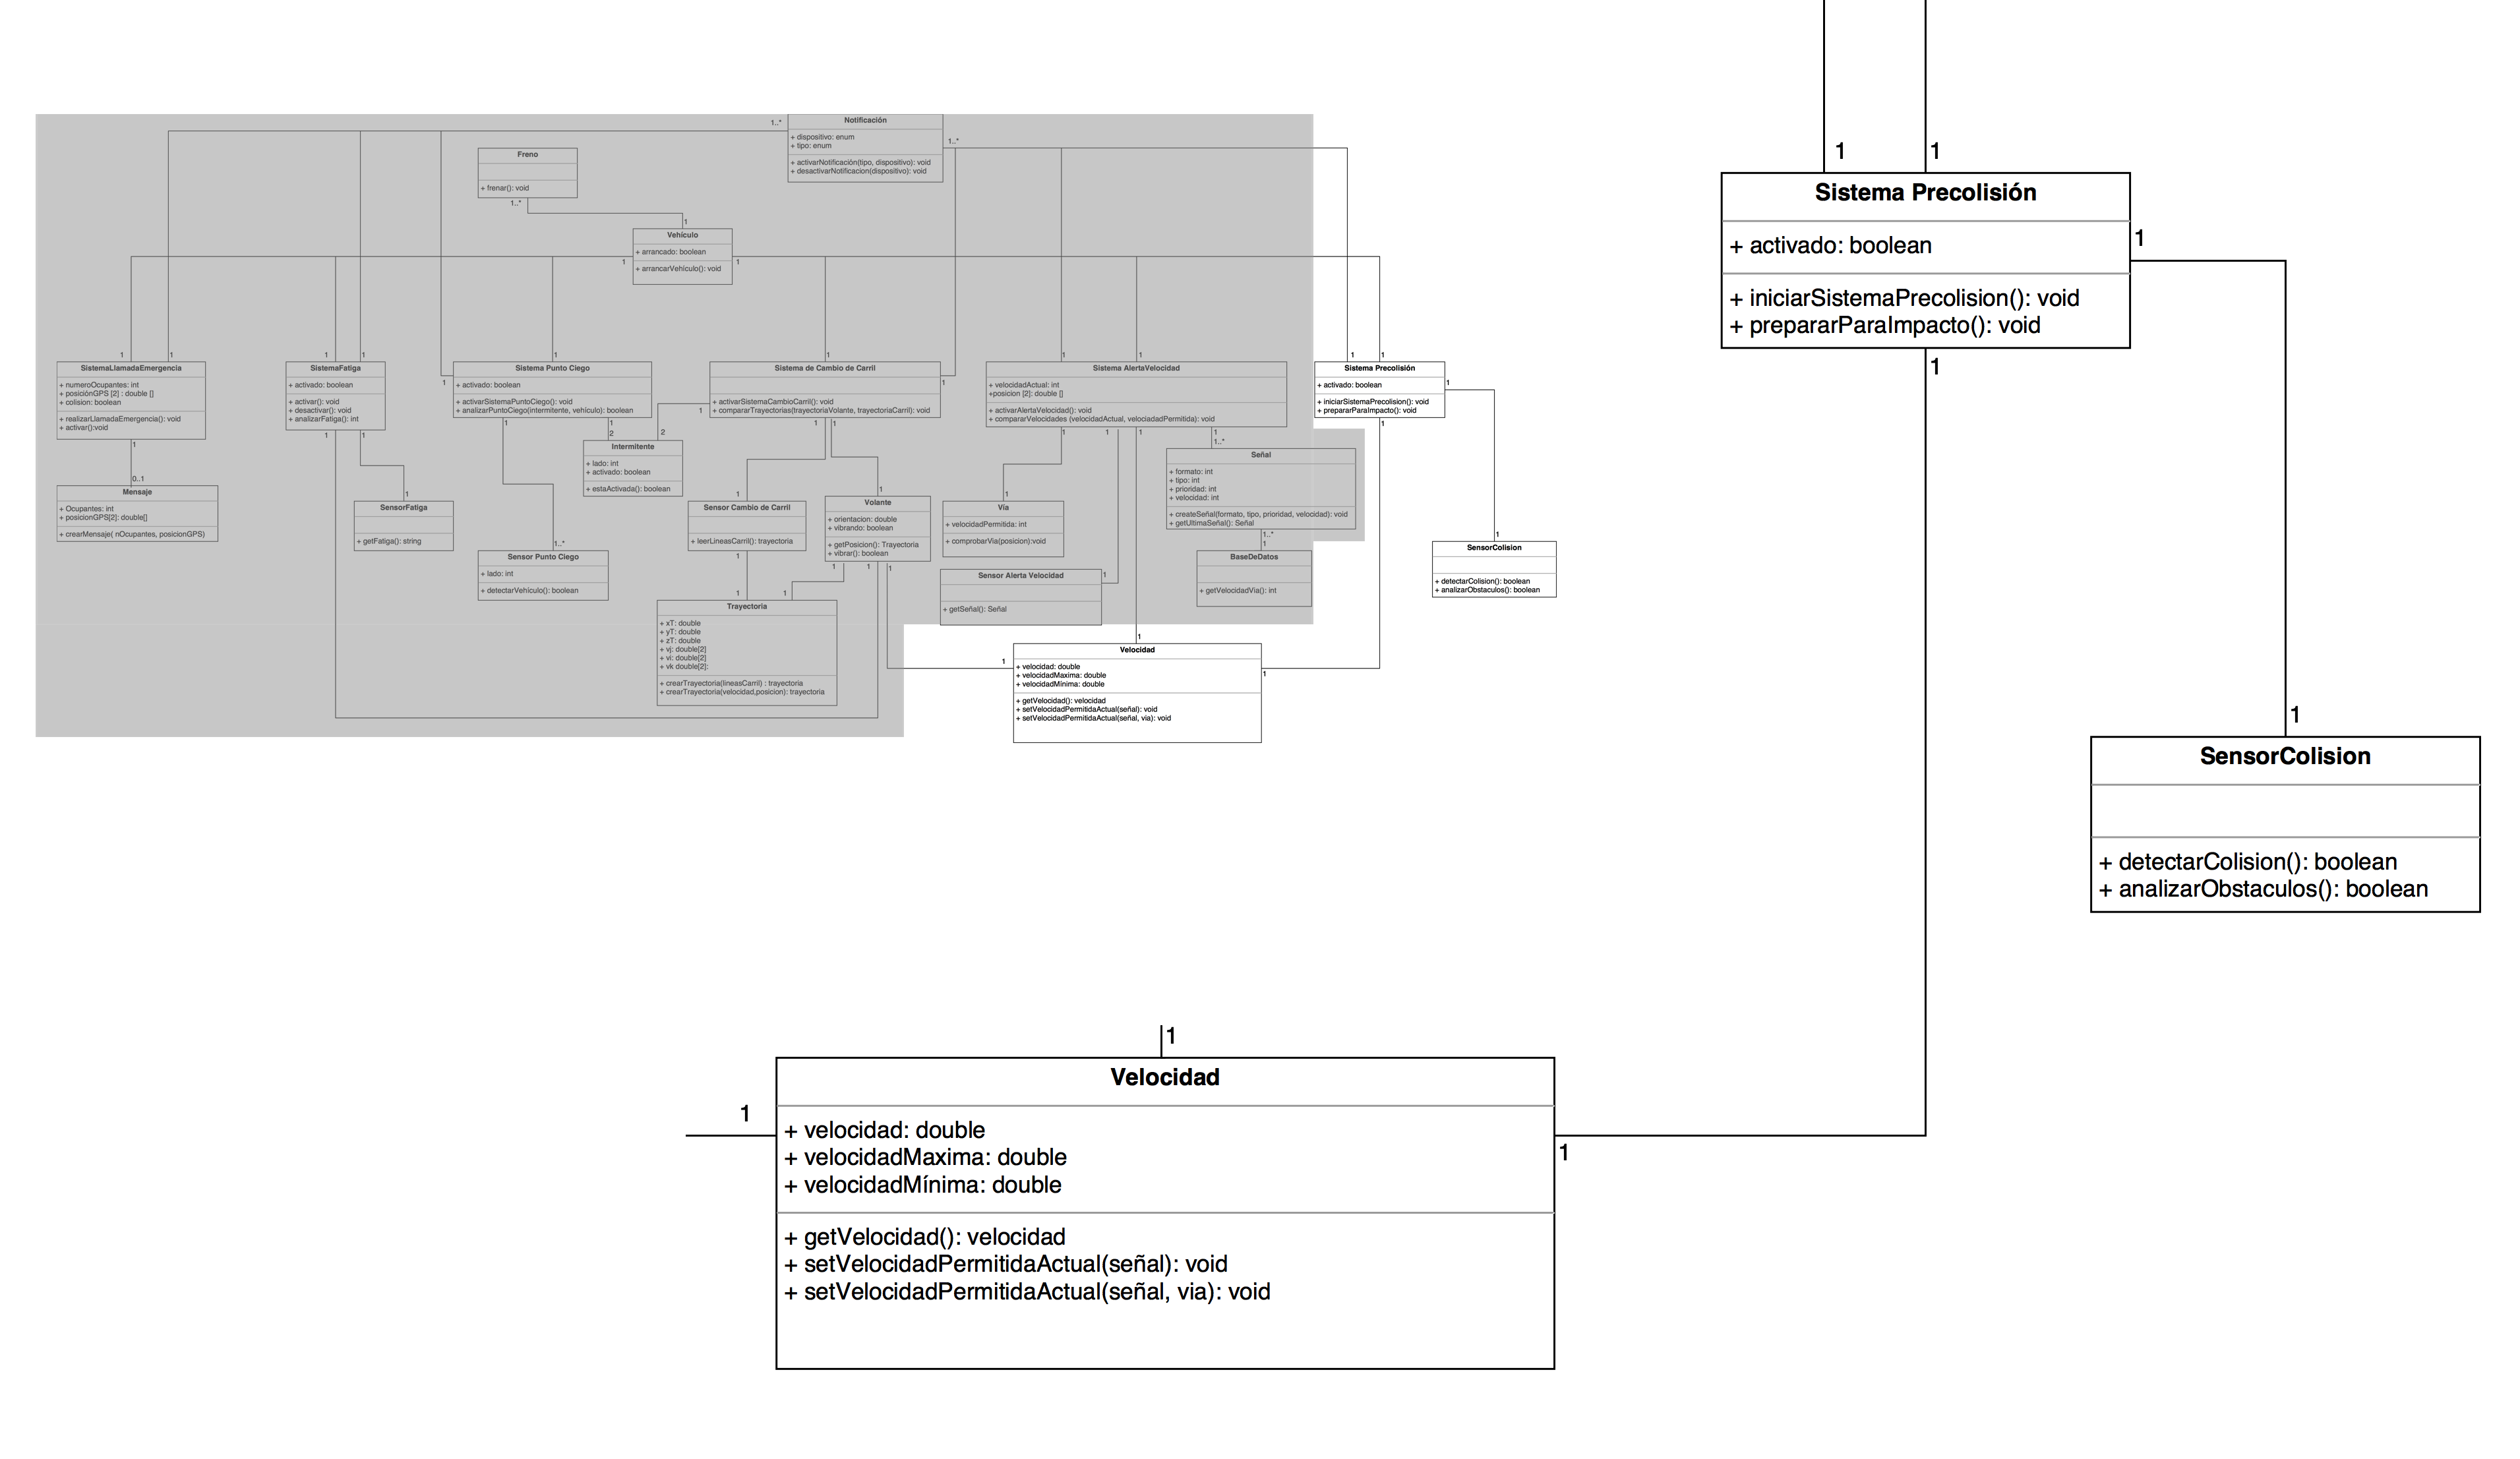
\includegraphics[width=1\textwidth]{./img/SistemaPrecolision.png}
\end{center}
\caption{Clases pertenecientes al subsistema SistemaPrecolision}
\label{tab:c_SistemaPrecolisionPNG}
\end{figure}



%Figura
\begin{figure}[H]
\begin{center}
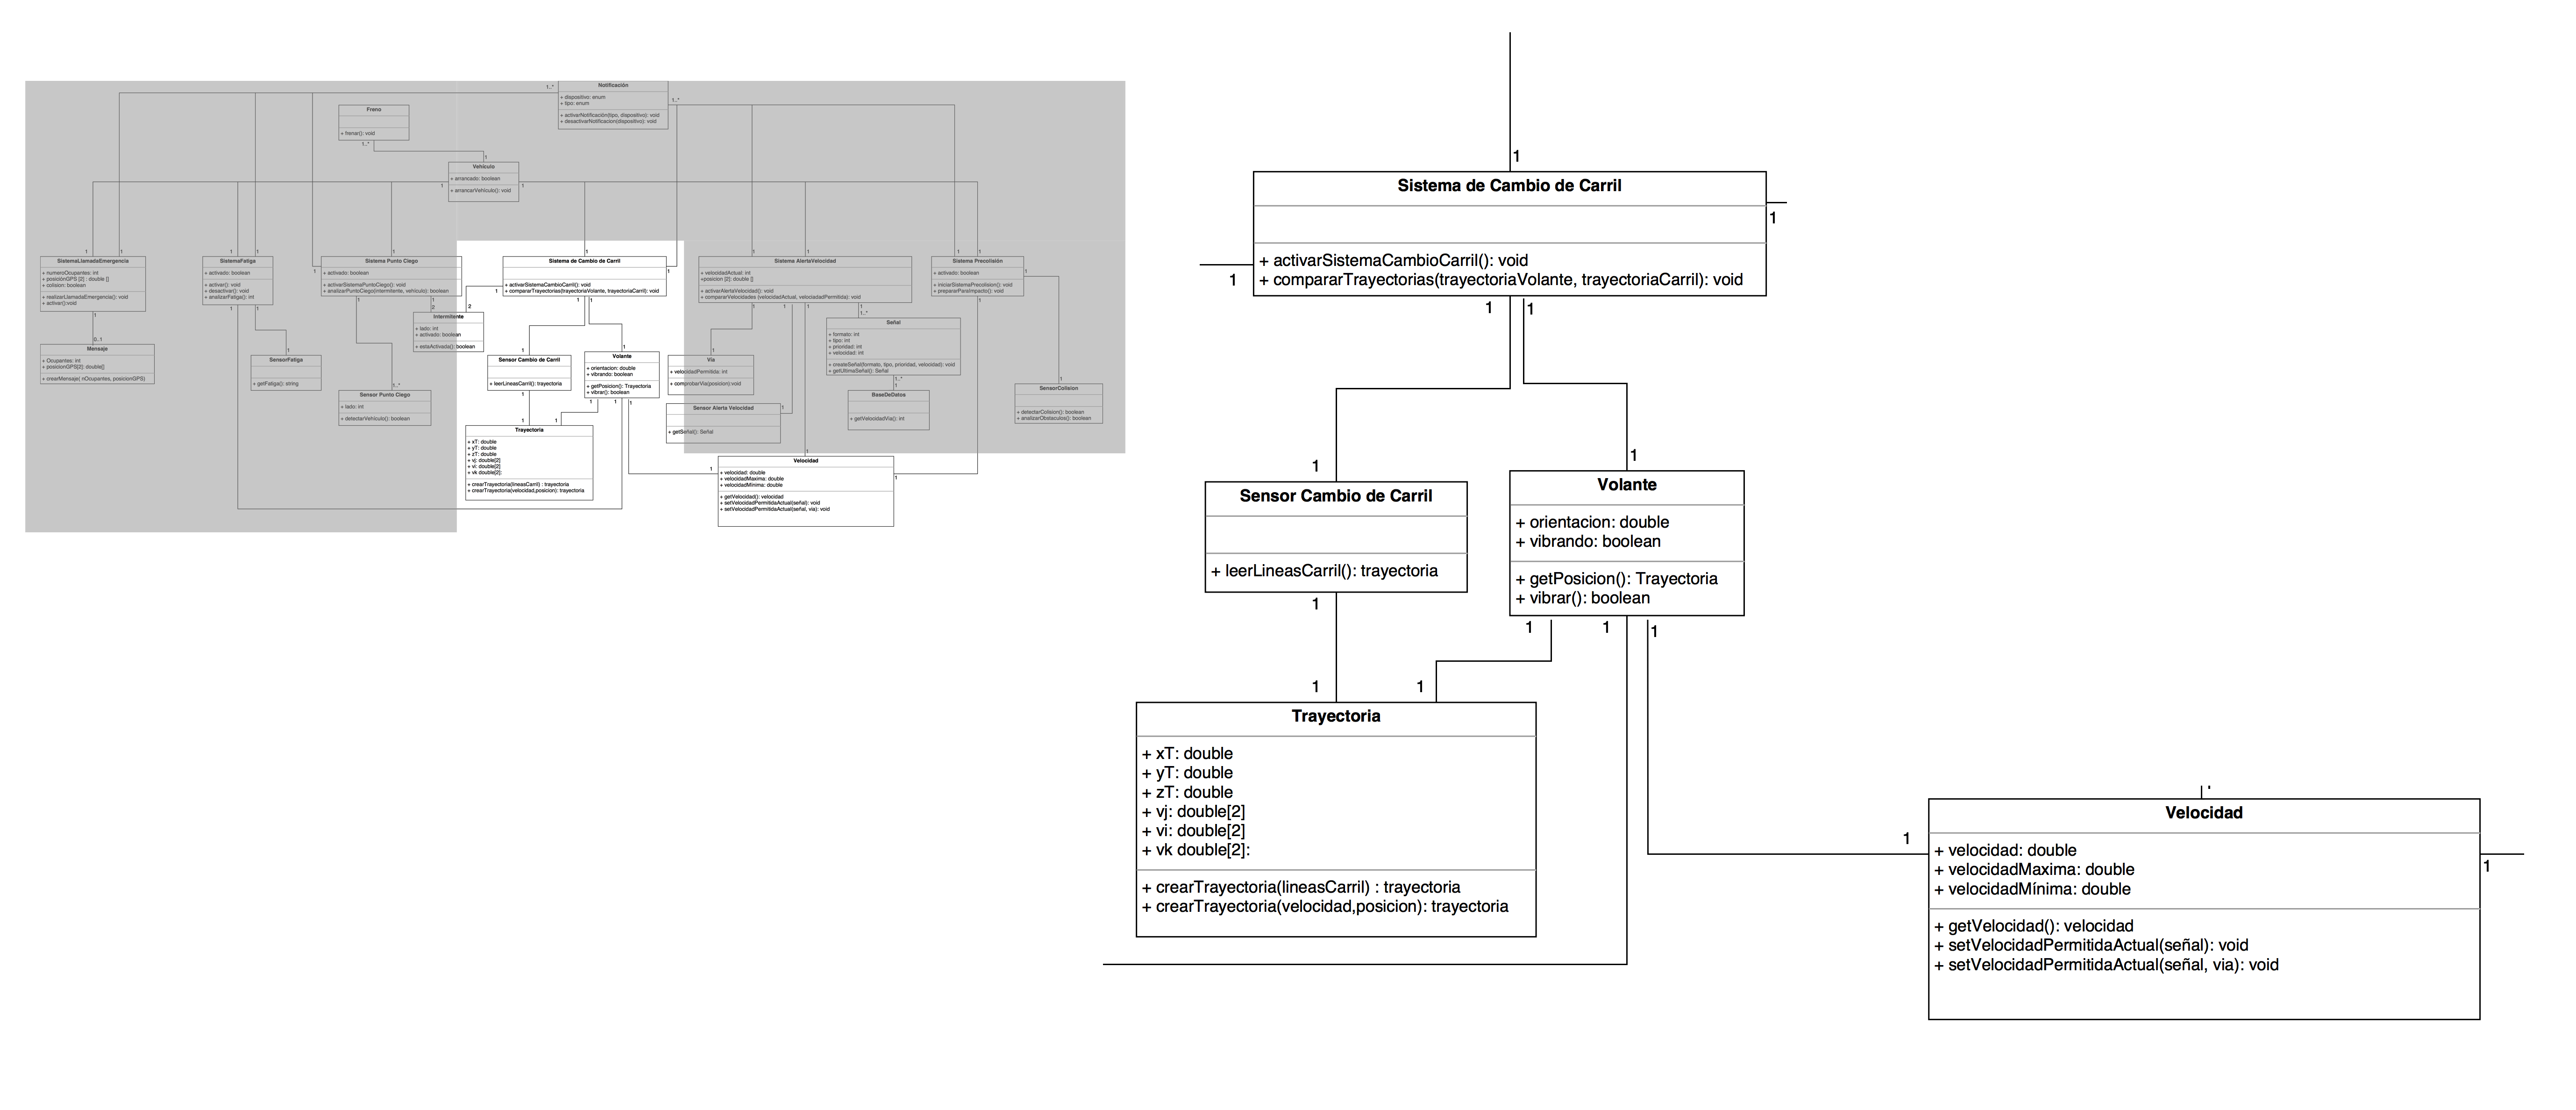
\includegraphics[width=1\textwidth]{./img/SistemaCambioCarril2.png}
\end{center}
\caption{Clases pertenecientes al subsistema SistemaCambioCarril}
\label{tab:c_SistemaCambioCarrilPNG}
\end{figure}




\par A continuación, se procede a explicar la funcionalidad de cada una de las clases representadas en el diagrama, junto con sus atributos y métodos asociados. Para ello se utilizará una tabla como la que se presenta a continuación:

\begin{table}[H]
\begin{center}
\begin{tabular}{p{3,5cm} p{11cm}}
\multicolumn{2}{c}{\textbf{Nombre de la clase} } \\ \hline \hline
\textbf{Responsabilidad} &  \\ \hline
\textbf{Atributos} &  \\ \hline
\textbf{Relaciones} & \\ \hline
\textbf{Métodos} &  \\ \hline
\end{tabular}
\caption{Formato de las tablas de las clases del modelo conceptual.}
\label{tab:formatoD_clases}
\end{center}
\end{table}

\par La explicación de cada uno de los campos analizados por la tabla \ref{tab:formatoD_clases} es el siguiente:
\begin{itemize}
  \item \textbf{Nombre de la clase}: nombre escogido que identifica inequivocamente la clase referenciada.
  \item \textbf{Responsabilidad}: descripción detallada de las acciones y responsabilidades que recaen sobre la clase.
  \item \textbf{Atributos}: enumeración de todos los atributos contenidos en la clase y que son necesarios para llevar a cabo las responsabilidades asociadas a la misma.
  \item \textbf{Relaciones}: relaciones con otras clases, ya sea de composición, agregación, asociación, etc.
  \item \textbf{Métodos}: métodos que se encuentran en la clase y que son necesarios para llevar a cabo las responsabilidades asociadas a la misma.
\end{itemize}









\begin{table}[H]
\begin{center}
\begin{tabular}{p{3,5cm} p{11cm}}
\multicolumn{2}{c}{\textbf{Vehículo} } \\ \hline \hline
\textbf{Responsabilidad} &  Encargada de arrancar todos los subsistemas de control y de gestionar la frenada del vehículo en caso de emergencia\\ \hline
\textbf{Atributos} &  \begin{itemize} \item arrancado: boolean \end{itemize}\\ \hline
\textbf{Relaciones} & Tiene una relación de composición con las siguientes clases:
                      \begin{itemize}
                        \item SistemaPuntoCiego \ref{tab:c_SPCiego}
                        \item SistemaCambioCarril \ref{tab:c_SCarril}
                        \item SistemaFatiga \ref{tab:c_SFatiga}
                        \item SistemaLlamadaEmergencia \ref{tab:c_SLEmerg}
                        \item SistemaPreColisión \ref{tab:c_SPColision}
                        \item SistemaAlertaVelocidad \ref{tab:c_SAVelocidad}
                        \item Freno \ref{tab:c_freno}
                      \end{itemize}\\ \hline
\textbf{Métodos} &  \begin{itemize}
                      \item arrancarVehiculo(): void
                    \end{itemize}\\ \hline
\end{tabular}
\caption{Clase Vehículo}
\label{tab:c_vehiculo}
\end{center}
\end{table}










\begin{table}[H]
\begin{center}
\begin{tabular}{p{3,5cm} p{11cm}}
\multicolumn{2}{c}{\textbf{SistemaPuntoCiego} } \\ \hline \hline
\textbf{Responsabilidad} &  Sistema encargado de procesar los datos recibidos por los diversos sensores que lo componen así como de decidir cuando se debe activar algún tipo de notificación para hacer saber al conductor que hay un objeto en el punto ciego del vehículo\\ \hline
\textbf{Atributos} &  \begin{itemize} \item activado: boolean \end{itemize}\\ \hline
\textbf{Relaciones} & \par Tiene una relación de composición con las siguientes clases:
                      \begin{itemize}
                        \item SensorPuntoCiego \ref{tab:c_SensorPC}
                        \item Vehículo \ref{tab:c_vehiculo}
                      \end{itemize}

                      \par Tiene una relación de agregación con las siguientes clases:
                        \begin{itemize}
                          \item Intermitente \ref{tab:c_Intermitente}
                        \end{itemize}

                      \par Tiene una relación de asociación con las siguientes clases:
                      \begin{itemize}
                        \item Notificación \ref{tab:c_Notificacion}
                      \end{itemize}\\ \hline

\textbf{Métodos} &  \begin{itemize}
                      \item activar(): void
                      \item desactivar(): void
                      \item analizarPuntoCiego(intermitente, vehiculo): boolean
                    \end{itemize}\\ \hline
\end{tabular}
\caption{Clase SistemaPuntoCiego}
\label{tab:c_SPCiego}
\end{center}
\end{table}









\begin{table}[H]
\begin{center}
\begin{tabular}{p{3,5cm} p{11cm}}
\multicolumn{2}{c}{\textbf{SensorPuntoCiego} } \\ \hline \hline
\textbf{Responsabilidad} &  Conjunto de sensores que detectan cuándo un objeto se encuentra situado en la zona del punto ciego del vehículo\\ \hline
\textbf{Atributos} &  \begin{itemize} \item lado: int \end{itemize}\\ \hline
\textbf{Relaciones} & \par Tiene una relación de composición con las siguientes clases:
                      \begin{itemize}
                        \item SistemaPuntoCiego \ref{tab:c_SPCiego}
                      \end{itemize}
                      \\ \hline

\textbf{Métodos} &  \begin{itemize}
                      \item detectarVehiculo(): boolean
                    \end{itemize}\\ \hline
\end{tabular}
\caption{Clase SensorPuntoCiego}
\label{tab:c_SensorPC}
\end{center}
\end{table}







\begin{table}[H]
\begin{center}
\begin{tabular}{p{3,5cm} p{11cm}}
\multicolumn{2}{c}{\textbf{Intermitente} } \\ \hline \hline
\textbf{Responsabilidad} &  Conjunto de intermitentes fisicos del vehiculo\\ \hline
\textbf{Atributos} &  \begin{itemize} \item lado: int \item activado: boolean \end{itemize}\\ \hline
\textbf{Relaciones} & \par Tiene una relación de agregación con las siguientes clases:
                      \begin{itemize}
                        \item SistemaPuntoCiego \ref{tab:c_SPCiego}
                        \item SistemaCambioCarril \ref{tab:c_SCarril}
                      \end{itemize}
                      \\ \hline

\textbf{Métodos} &  \begin{itemize}
                      \item estaActivada(): boolean
                    \end{itemize}\\ \hline
\end{tabular}
\caption{Clase Intermitente}
\label{tab:c_Intermitente}
\end{center}
\end{table}








\begin{table}[H]
\begin{center}
\begin{tabular}{p{3,5cm} p{11cm}}
\multicolumn{2}{c}{\textbf{SistemaCambioCarril} } \\ \hline \hline
\textbf{Responsabilidad} &  Sistema encargado de procesar los datos recibidos por los diversos sensores que lo componen para poder calcular la desviación respecto al carril que va a seguir el vehículo, así como hacer vibrar o mover el volante para permanecer en el carril por el se circula y decidir cuando se debe activar algún tipo de notificación para hacer saber al conductor del vehículo que se está saliendo del carril. \\ \hline
\textbf{Atributos} & No contiene atributos
                      \\ \hline
\textbf{Relaciones} &

                      \par Tiene una relación de composición con las siguientes clases:
                      \begin{itemize}
                        \item Vehículo \ref{tab:c_vehiculo}
                        \item SensorCambioCarril \ref{tab:c_SensorCC}
                      \end{itemize}

                      \par Tiene una relación de agregación con las siguientes clases:
                        \begin{itemize}
                          \item Volante \ref{tab:c_Volante}
                          \item Intermitente \ref{tab:c_Intermitente}
                        \end{itemize}

                        \par Tiene una relación de asociación con las siguientes clases:
                        \begin{itemize}
                          \item Notificación \ref{tab:c_Notificacion}
                        \end{itemize}

                      \\ \hline

\textbf{Métodos} &  \begin{itemize}
                      \item activar(): void
                      \item desactivar(): void
                      \item compararTrayectorias(trayectoriaVolante, trayectoriaCarril): void
                    \end{itemize}\\ \hline
\end{tabular}
\caption{Clase SistemaCambioCarril}
\label{tab:c_SCarril}
\end{center}
\end{table}









\begin{table}[H]
\begin{center}
\begin{tabular}{p{3,5cm} p{11cm}}
\multicolumn{2}{c}{\textbf{SensorCambioCarril} } \\ \hline \hline
\textbf{Responsabilidad} &  Conjunto de sensores que detectan la trayectoria del carril por el que se encuentra circulando el vehículo. \\ \hline
\textbf{Atributos} & No contiene atributos
                      \\ \hline
\textbf{Relaciones} & \par Tiene una relación de composición con las siguientes clases:
                      \begin{itemize}
                        \item SistemaCambioCarril \ref{tab:c_SCarril}
                      \end{itemize}

                      \par Tiene una relación de agregación con las siguientes clases:
                      \begin{itemize}
                        \item Trayectoria \ref{tab:c_trayectoria}
                      \end{itemize}
                      \\ \hline

\textbf{Métodos} &  \begin{itemize}
                      \item leerLineasCarril(): trayectoria
                      \end{itemize}\\ \hline
\end{tabular}
\caption{Clase SensorCambioCarril}
\label{tab:c_SensorCC}
\end{center}
\end{table}








\begin{table}[H]
\begin{center}
\begin{tabular}{p{3,5cm} p{11cm}}
\multicolumn{2}{c}{\textbf{Trayectoria} } \\ \hline \hline
\textbf{Responsabilidad} &  Trayectoria detectada\\ \hline
\textbf{Atributos} &  \begin{itemize}
                        \item xT: double
                        \item yT: double
                        \item zT: double
                        \item vi: double[2]
                        \item vj: double[2]
                        \item vk: double[2]
                      \end{itemize}
                      \\ \hline
\textbf{Relaciones} & \par Tiene una relación de agregación con las siguientes clases:
                      \begin{itemize}
                        \item SensorCambioCarril \ref{tab:c_SensorCC}
                        \item Volante \ref{tab:c_Volante}
                      \end{itemize}
                      \\ \hline

\textbf{Métodos} &  \begin{itemize}
                      \item generarTrayectoria(lineasCarril): trayectoria
                      \item generarTrayectoria(velocidad, posicion): trayectoria
                    \end{itemize}\\ \hline
\end{tabular}
\caption{Clase Trayectoria}
\label{tab:c_trayectoria}
\end{center}
\end{table}









\begin{table}[H]
\begin{center}
\begin{tabular}{p{3,5cm} p{11cm}}
\multicolumn{2}{c}{\textbf{Volante} } \\ \hline \hline
\textbf{Responsabilidad} &  Clase que recopila información sobre la posición del volante y con la capacidad de hacer vibrar al mismo.  \\ \hline
\textbf{Atributos} & \begin{itemize}
                      \item orientacion: double
                      \item vibrando: boolean
                    \end{itemize}
                      \\ \hline
\textbf{Relaciones} & \par Tiene una relación de composición con las siguientes clases:
                      \begin{itemize}
                        \item SistemaCambioCarril \ref{tab:c_SCarril}
                      \end{itemize}

                      \par Tiene una relación de agregación con las siguientes clases:
                      \begin{itemize}
                        \item Velocidad \ref{tab:c_velocidad}
                        \item Trayectoria \ref{tab:c_trayectoria}
                      \end{itemize}

                      \par Tiene una relación de asociación con las siguientes clases:
                      \begin{itemize}
                        \item SistemaFatiga \ref{tab:c_SFatiga}
                      \end{itemize}

                      \\ \hline



\textbf{Métodos} &  \begin{itemize}
                      \item getPosicion(): trayectoria
                      \item vibrar(): boolean
                    \end{itemize}\\ \hline
\end{tabular}
\caption{Clase Volante}
\label{tab:c_Volante}
\end{center}
\end{table}









\begin{table}[H]
\begin{center}
\begin{tabular}{p{3,5cm} p{11cm}}
\multicolumn{2}{c}{\textbf{SistemaAlertaVelocidad} } \\ \hline \hline
\textbf{Responsabilidad} &  Sistema encargado de gestionar la velocidad máxima para la vía por la que el vehículo se encuentra circulando, en todo momento.  \\ \hline
\textbf{Atributos} & \begin{itemize}
                      \item velocidadActual: int
                      \item posicion[2]: double []
                    \end{itemize}\\ \hline
\textbf{Relaciones} & \par Tiene una relación de composición con las siguientes clases:
                      \begin{itemize}
                        \item SensorAlertaVelocidad \ref{tab:c_SensorAV}
                        \item Vía \ref{tab:c_via}
                        \item Vehículo \ref{tab:c_vehiculo}
                      \end{itemize}

                      \par Tiene una relación de agregación con las siguientes clases:
                      \begin{itemize}
                        \item Señal \ref{tab:c_senal}
                        \item Velocidad \ref{tab:c_velocidad}
                      \end{itemize}

                      \par Tiene una relación de asociación con las siguientes clases:
                      \begin{itemize}
                        \item Notificación \ref{tab:c_Notificacion}
                      \end{itemize}

                      \\ \hline

\textbf{Métodos} &  \begin{itemize}
                      \item activar(): void
                      \item desactivar(): void
                      \item compararVelocidades(velocidadActual, velocidadPermitida): void
                    \end{itemize}\\ \hline
\end{tabular}
\caption{Clase SistemaAlertaVelocidad}
\label{tab:c_SAVelocidad}
\end{center}
\end{table}








\begin{table}[H]
\begin{center}
\begin{tabular}{p{3,5cm} p{11cm}}
\multicolumn{2}{c}{\textbf{Vía} } \\ \hline \hline
\textbf{Responsabilidad} &  Clase que debe comprobar en qué tipo de vía se encuentra el vehículo y determinar de esta forma la velocidad máxima permitida.  \\ \hline
\textbf{Atributos} & \begin{itemize}
                      \item velocidadPermitida: int
                    \end{itemize}\\ \hline
\textbf{Relaciones} & \par Tiene una relación de composición con las siguientes clases:
                      \begin{itemize}
                        \item SistemaAlertaVelocidad \ref{tab:c_SAVelocidad}
                        \item BaseDeDatos \ref{tab:c_bbdd}
                      \end{itemize}

                      \\ \hline

\textbf{Métodos} &  \begin{itemize}
                      \item comprobarVia(posición): void
                    \end{itemize}\\ \hline
\end{tabular}
\caption{Clase Vía}
\label{tab:c_via}
\end{center}
\end{table}








\begin{table}[H]
\begin{center}
\begin{tabular}{p{3,5cm} p{11cm}}
\multicolumn{2}{c}{\textbf{BaseDeDatos} } \\ \hline \hline
\textbf{Responsabilidad} &  Clase encargada de almacenar toda la información referente a los tipos de vía existentes y las velocidades máximas a las que está permitido circular en las mismas.   \\ \hline
\textbf{Atributos} & Esta clase no tiene atributos\\ \hline
\textbf{Relaciones} & \par Tiene una relación de composición con las siguientes clases:
                      \begin{itemize}
                        \item Vía \ref{tab:c_via}
                      \end{itemize}



                      \\ \hline

\textbf{Métodos} &  \begin{itemize}
                      \item getVelocidadVia(): int
                      \end{itemize}\\ \hline
\end{tabular}
\caption{Clase BaseDeDatos}
\label{tab:c_bbdd}
\end{center}
\end{table}









\begin{table}[H]
\begin{center}
\begin{tabular}{p{3,5cm} p{11cm}}
\multicolumn{2}{c}{\textbf{SensorAlertaVelocidad} } \\ \hline \hline
\textbf{Responsabilidad} &  Clase encargada de detectar las señales de trafico.   \\ \hline
\textbf{Atributos} & Esta clase no tiene atributos\\ \hline
\textbf{Relaciones} & \par Tiene una relación de composición con las siguientes clases:
                      \begin{itemize}
                        \item SistemaAlertaVelocidad \ref{tab:c_SAVelocidad}
                      \end{itemize}

                      \par Tiene una relación de agregación con las siguientes clases:
                      \begin{itemize}
                        \item Señal \ref{tab:c_senal}
                      \end{itemize}

                      \\ \hline

\textbf{Métodos} &  \begin{itemize}
                      \item getSeñal(): señal
                      \end{itemize}\\ \hline
\end{tabular}
\caption{Clase SensorAlertaVelocidad}
\label{tab:c_SensorAV}
\end{center}
\end{table}









\begin{table}[H]
\begin{center}
\begin{tabular}{p{3,5cm} p{11cm}}
\multicolumn{2}{c}{\textbf{Señal} } \\ \hline \hline
\textbf{Responsabilidad} &  Clase que crea y almacena la informacion obtenida por una lectura de una señal de tráfico. \\ \hline
\textbf{Atributos} & \begin{itemize}
                      \item formato: int
                      \item tipo: int
                      \item prioridad: int
                      \item velocidad: int

                    \end{itemize}\\ \hline
\textbf{Relaciones} &

                      \par Tiene una relación de agregación con las siguientes clases:
                      \begin{itemize}
                        \item SensorAlertaVelocidad \ref{tab:c_SensorAV}
                        \item SistemaAlertaVelocidad \ref{tab:c_SAVelocidad}
                      \end{itemize}



                      \\ \hline

\textbf{Métodos} &  \begin{itemize}
                      \item createSeñal(formato, tipo, prioridad, velocidad): void
                      \item getUltimaSeñal(): señal
                    \end{itemize}\\ \hline
\end{tabular}
\caption{Clase Señal}
\label{tab:c_senal}
\end{center}
\end{table}










\begin{table}[H]
\begin{center}
\begin{tabular}{p{3,5cm} p{11cm}}
\multicolumn{2}{c}{\textbf{Velocidad} } \\ \hline \hline
\textbf{Responsabilidad} &  Clase encargada de obtener la velocidad a la que circula el vehículo y de fijar la velocidad máxima a la que se puede circular en función de una señal o del tipo de vía en la que se encuentre circulando el vehículo.  \\ \hline
\textbf{Atributos} & \begin{itemize}
                      \item velocidad: double
                      \item velocidadMáxima: double
                      \item velocidadMínima: double

                    \end{itemize}\\ \hline
\textbf{Relaciones} &

                      \par Tiene una relación de agregación con las siguientes clases:
                      \begin{itemize}
                        \item Volante \ref{tab:c_Volante}
                        \item SistemaAlertaVelocidad \ref{tab:c_SAVelocidad}
                        \item SistemaPreColisión \ref{tab:c_SPColision}
                      \end{itemize}



                      \\ \hline

\textbf{Métodos} &  \begin{itemize}
                      \item getVelocidad(): velocidad
                      \item setVelocidadPermitidaActual(señal): void
                      \item setVelocidadPermitidaActual(señal, via): void
                    \end{itemize}\\ \hline
\end{tabular}
\caption{Clase Velocidad}
\label{tab:c_velocidad}
\end{center}
\end{table}












\begin{table}[H]
\begin{center}
\begin{tabular}{p{3,5cm} p{11cm}}
\multicolumn{2}{c}{\textbf{SistemaPreColisión} } \\ \hline \hline
\textbf{Responsabilidad} &  Sistema encargado de detectar cuando el vehículo se encuentra en riesgo de sufrir una colisión, solicitar la activación de una notificación y preparar el vehículo para el impacto.  \\ \hline
\textbf{Atributos} & \begin{itemize}
                      \item activado: boolean
                    \end{itemize}\\ \hline
\textbf{Relaciones} & \par Tiene una relación de composición con las siguientes clases:
                      \begin{itemize}
                        \item Vehículo \ref{tab:c_vehiculo}
                        \item SensorColisión \ref{tab:c_SensorC}
                      \end{itemize}

                      \par Tiene una relación de agregación con las siguientes clases:
                      \begin{itemize}
                        \item Velocidad \ref{tab:c_velocidad}
                      \end{itemize}

                      \par Tiene una relación de asociación con las siguientes clases:
                      \begin{itemize}
                        \item Notificación \ref{tab:c_Notificacion}
                      \end{itemize}


                      \\ \hline

\textbf{Métodos} &  \begin{itemize}
                      \item activar(): void
                      \item desactivar(): void
                      \item prepararParaImpacto(): void
                    \end{itemize}\\ \hline
\end{tabular}
\caption{Clase SistemaPreColisión}
\label{tab:c_SPColision}
\end{center}
\end{table}









\begin{table}[H]
\begin{center}
\begin{tabular}{p{3,5cm} p{11cm}}
\multicolumn{2}{c}{\textbf{SensorColisión} } \\ \hline \hline
\textbf{Responsabilidad} &  Conjunto de sensores que deben detectar cuando hay un objeto en la trayectoria del vehículo que sea susceptible de generar una colisión  \\ \hline
\textbf{Atributos} & Esta clase no contiene atributos\\ \hline
\textbf{Relaciones} & \par Tiene una relación de composición con las siguientes clases:
                      \begin{itemize}
                        \item SistemaPreColisión \ref{tab:c_SPColision}
                      \end{itemize}

                      \\ \hline

\textbf{Métodos} &  \begin{itemize}
                      \item detectarColisión(): void
                      \item analizarObstaculos(): void
                    \end{itemize}\\ \hline
\end{tabular}
\caption{Clase SensorColisión}
\label{tab:c_SensorC}
\end{center}
\end{table}








\begin{table}[H]
\begin{center}
\begin{tabular}{p{3,5cm} p{11cm}}
\multicolumn{2}{c}{\textbf{SistemaFatiga} } \\ \hline \hline
\textbf{Responsabilidad} &  Sistema encargado de analizar la situación física en la que se encuentra el conductor del vehículo. Deberá analizar la posición de los parpados la presión ejercida sobre el volante, tomando las acciones oportunas en caso de emergencia.  \\ \hline
\textbf{Atributos} & \begin{itemize}
                      \item activado: boolean
                    \end{itemize}\\ \hline
\textbf{Relaciones} & \par Tiene una relación de composición con las siguientes clases:
                      \begin{itemize}
                        \item Vehículo \ref{tab:c_vehiculo}
                        \item SensorFatiga \ref{tab:c_SensorF}
                      \end{itemize}

                      \par Tiene una relación de agregación con las siguientes clases:
                      \begin{itemize}
                        \item Volante \ref{tab:c_Volante}
                      \end{itemize}

                      \par Tiene una relación de asociación con las siguientes clases:
                      \begin{itemize}
                        \item Notificación \ref{tab:c_Notificacion}
                      \end{itemize}


                      \\ \hline

\textbf{Métodos} &  \begin{itemize}
                      \item activar(): void
                      \item desactivar(): void
                      \item analizarFatiga(): void
                    \end{itemize}\\ \hline
\end{tabular}
\caption{Clase SistemaFatiga}
\label{tab:c_SFatiga}
\end{center}
\end{table}











\begin{table}[H]
\begin{center}
\begin{tabular}{p{3,5cm} p{11cm}}
\multicolumn{2}{c}{\textbf{SensorFatiga} } \\ \hline \hline
\textbf{Responsabilidad} &  Conjunto de sensores que deben detectar cuando el conductor del vehículo se está quedando o dormido o ha perdido la concentración en la carretera.  \\ \hline
\textbf{Atributos} & Esta clase no contiene atributos\\ \hline
\textbf{Relaciones} & \par Tiene una relación de composición con las siguientes clases:
                      \begin{itemize}
                        \item SistemaPreColisión \ref{tab:c_SFatiga}
                      \end{itemize}

                      \\ \hline

\textbf{Métodos} &  \begin{itemize}
                      \item getFatiga(): string
                    \end{itemize}\\ \hline
\end{tabular}
\caption{Clase SensorFatiga}
\label{tab:c_SensorF}
\end{center}
\end{table}









\begin{table}[H]
\begin{center}
\begin{tabular}{p{3,5cm} p{11cm}}
\multicolumn{2}{c}{\textbf{SistemaLlamadaEmergencia} } \\ \hline \hline
\textbf{Responsabilidad} &  Sistema encargado de realizar una llamada de emergencia cuando ha ocurrido un accidente.  \\ \hline
\textbf{Atributos} & \begin{itemize}
                      \item numeroOcupantes: int
                      \item posicionGPS[2]: double[]
                      \item colision: boolean
                    \end{itemize}\\ \hline
\textbf{Relaciones} & \par Tiene una relación de composición con las siguientes clases:
                      \begin{itemize}
                        \item Vehículo \ref{tab:c_vehiculo}
                        \item Mensaje \ref{tab:c_mensaje}
                      \end{itemize}

                      \par Tiene una relación de agregación con las siguientes clases:
                      \begin{itemize}
                        \item Volante \ref{tab:c_Volante}
                      \end{itemize}

                      \par Tiene una relación de asociación con las siguientes clases:
                      \begin{itemize}
                        \item Notificación \ref{tab:c_Notificacion}
                      \end{itemize}


                      \\ \hline

\textbf{Métodos} &  \begin{itemize}
                      \item activar(): void
                      \item desactivar(): void
                      \item enviarMensaje(): void
                    \end{itemize}\\ \hline
\end{tabular}
\caption{Clase SistemaLlamadaEmergencia}
\label{tab:c_SLEmerg}
\end{center}
\end{table}










\begin{table}[H]
\begin{center}
\begin{tabular}{p{3,5cm} p{11cm}}
\multicolumn{2}{c}{\textbf{Mensaje} } \\ \hline \hline
\textbf{Responsabilidad} &   Clase encargada de generar el mensaje que posteriormente será enviado por la clase SistemaLlamadaEmergencia \ref{tab:c_SLEmerg}  \\ \hline
\textbf{Atributos} & \begin{itemize}
                      \item Ocupantes: int
                      \item posicionGPS[2]: double[]
                    \end{itemize}\\ \hline
\textbf{Relaciones} & \par Tiene una relación de composición con las siguientes clases:
                      \begin{itemize}
                        \item SistemaLlamadaEmergencia \ref{tab:c_SLEmerg}
                      \end{itemize}

                      \\ \hline

\textbf{Métodos} &  \begin{itemize}
                      \item crearMensaje(): string
                    \end{itemize}\\ \hline
\end{tabular}
\caption{Clase Mensaje}
\label{tab:c_mensaje}
\end{center}
\end{table}






\begin{table}[H]
\begin{center}
\begin{tabular}{p{3,5cm} p{11cm}}
\multicolumn{2}{c}{\textbf{Freno} } \\ \hline \hline
\textbf{Responsabilidad} &   Clase encargada de accionar el freno fisico del vehículo en caso de emergencia  \\ \hline
\textbf{Atributos} & Esta clase no contiene atributos\\ \hline
\textbf{Relaciones} & \par Tiene una relación de composición con las siguientes clases:
                      \begin{itemize}
                        \item Vehículo \ref{tab:c_vehiculo}
                      \end{itemize}

                      \\ \hline

\textbf{Métodos} &  \begin{itemize}
                      \item frenar(): void
                    \end{itemize}\\ \hline
\end{tabular}
\caption{Clase Freno}
\label{tab:c_freno}
\end{center}
\end{table}








\begin{table}[H]
\begin{center}
\begin{tabular}{p{3,5cm} p{11cm}}
\multicolumn{2}{c}{\textbf{Notificación} } \\ \hline \hline
\textbf{Responsabilidad} &   Clase encargada de generar, activar y desactivar todas las notificaciones del sistema. Para ello necesitará saber el dispositivo que solicita la notificación y el tipo de la misma  \\ \hline
\textbf{Atributos} & \begin{itemize}
                      \item dispositivo: enum
                      \item tipo: enum
                    \end{itemize}\\ \hline
\textbf{Relaciones} & \par Tiene una relación de composición con las siguientes clases:
                      \begin{itemize}
                        \item Vehículo \ref{tab:c_vehiculo}
                      \end{itemize}

                      \par Tiene una relación de asociación con las siguientes clases:
                      \begin{itemize}
                        \item SistemaPuntoCiego \ref{tab:c_SPCiego}
                        \item SistemaCambioCarril \ref{tab:c_SCarril}
                        \item SistemaFatiga \ref{tab:c_SFatiga}
                        \item SistemaLlamadaEmergencia \ref{tab:c_SLEmerg}
                        \item SistemaPreColisión \ref{tab:c_SPColision}
                        \item SistemaAlertaVelocidad \ref{tab:c_SAVelocidad}
                      \end{itemize}

                      \\ \hline

\textbf{Métodos} &  \begin{itemize}
                      \item activarNotificacion(tipo, dispositivo): void
                      \item desactivarNotificacion(tipo, dispositivo): void
                    \end{itemize}\\ \hline
\end{tabular}
\caption{Clase Notificación}
\label{tab:c_Notificacion}
\end{center}
\end{table}
